\chapter{Experimental Evaluation}\label{sec-eval}
In this chapter, we evaluate Mars on a single machine using a micro-benchmark of six applications in comparison with their CPU-based counterparts and native GPU-based implementations.
\red{We also evaluate the performance of MarsHadoop on two connected machines.}


\section{Experimental Setup}
Our experiments were performed on three PCs, A, B and
 C. Table \ref{tb:machines} shows their hardware configuration.
Both PCs A and B run 32-bit CentOS 5.1 Linux with kernel
2.6.18, NVIDIA CUDA 2.2, and the GPU driver 185.18.14. PC C runs
32-bit Windows XP Pro SP3, with Brook+ 1.01.0 beta, and the GPU
driver 8.561. All hard drives on these PCs are SATA magnetic hard
disks with 7200 rpm. On all PCs, the main memory and the device
memory are connected by PCI-E bus with a theoretical bandwidth of 4
GB/sec.

\doublerulesep 0.1pt
\begin{table}[htb]
  \centering
 \linespread{1.7}{ {\footnotesize
  \caption{Machine configurations}\label{tb:machines}
\vspace{2em}
  \begin{tabular}{p{4.5cm}p{3.5cm}p{3.5cm}p{3.5cm}}
  \hline
\noalign{\smallskip}
    \textbf{Machine} & \textbf{PC A}&\textbf{PC B}&\textbf{PC C}\\
\noalign{\smallskip}
  \hline
    GPU&NVIDIA GTX280& NVIDIA 8800GTX & ATI Radeon HD 3870\\
    \# GPU core & 240 & 128 & 320 \\
    GPU Core Clock (MHz)&602&575&775 \\
    GPU Memory Clock (MHz)&1107&900&2250 \\
    GPU Memory Bandwidth (GB/s)& 141.7& 86.4 &72.0\\
    GPU Memory Capacity (MB)& 1024 & 768 & 512\\
    CPU&Intel Core2 Quad Q6600 & Intel Core2 Quad Q6600 & Intel Pentium 4 540 \\
    CPU Clock (MHz)&2400&2400&3200 \\
    \# CPU core& 4 & 4 & 2\\
    CPU Memory Capacity (MB)& 2048 & 2048 & 1024\\
   \hline
 \hline
\noalign{\smallskip}
  \end{tabular}
  }}
\end{table}



\section{Micro-benchmark}

We have implemented the following six real-world applications for
evaluating the MapReduce framework.

{\bf String Match (SM):} Each Map task searches a portion of the
input file to check whether the target string is in the portion.
Neither the {\em Group} nor the {\em Reduce} stage is needed.
%The three data sets include 5 million, 10 million, and 15 million text lines to match respectively.

{\bf Matrix Multiplication (MM):} Matrix multiplication is used
intensively in analyzing the relationship of two documents. Given two
matrices $M$ and $N$, each Map task computes multiplication for a
row from $M$ and a column from $N$. It outputs the pair of the row
ID and the column ID as the key and the corresponding result as the
value. Neither the {\em Group} nor the {\em Reduce} stage is needed.
%The three data sets include about 65 thousand, 262 thousand, and 1 million pairs of row and column multiplications respectively.


{\bf Black-Scholes:} Black-Scholes model~\cite{Black1973} is used for calculating the price for European options according to a partial differential equation.
For each option, a Map task computes the prices for the call and put prices of an option, and emits a structure containing the price of the option call and the price of the option put as the key, and the option id as the value. The Group stage is to rank the price of option calls. No Reduce stage is needed.


{\bf Similarity Score (SS):} It is used in web document clustering.
The characteristics of a document are represented using a feature
vector of floating point numbers. Given two document features,
$\vec{a}$ and $\vec{b}$, the similarity score between these two
documents is defined to be $\frac{\vec{a}\cdot
\vec{b}}{|\vec{a}|\cdot |\vec{b}|}$. SS computes the pair-wise
similarity score for a set of documents. Each Map task computes the
similarity score for two documents. It outputs the intermediate pair
with the score as the key and the pair of the two document IDs as the
value. The {\em Group} stage is required to rank the pair-wise similarity
scores and no {\em Reduce} stage is required. %The three data sets include
%about 130 thousand, 262 thousand, and 1 million pairs of document
%features for calculation respectively.

\red{
{\bf Principal component analysis (PCA):} This application computes the mean vector and the covariance matrix of a set of points in the first two steps in PCA.
The input data is stored in a matrix.
The whole process contains two MapReduce invocations in a chain.
The first MapReduce procedure is to find the mean for each row in the matrix, and the second is to calculate the covariance matrix.
Neither Group nor Reduce stage is needed in the first MapReduce invocation. A Map task computes the mean for a row. In the second invocation, each Map task is to calculate the covariance of two rows.
The Group stage is required to sort the row-pairs by row IDs.
No Reduce phase is needed.
}


{\bf Monte Carlo (MC):} Monte Carlo~\cite{Boyle1977} is used to compute option pricing in financial engineering.
The Monte Carlo numeric integration is to mathematically estimate the expectation of the price of option call.
Each Map task is to compute the expected value of a random sample for an option, and to emit the option ID as the key, while the expected value of the random sample as the value.
The Group stage and the Reduce stage are required to calculate the mean of all the samples for each option.
In this application, all the options have the same number of samples, and the intermediate results are ordered by option ID already. Mars does not need to perform sorting in the Group stage.

The above applications are commonly used in benchmarking MapReduce implementations in the previous studies~\cite{Chu2006, Ranger2007}. SM, MM and PCA are adopted from Phoenix suite \cite{Ranger2007},  SS is a common component in web applications,
while BS and MC are prevalent in financial engineering, and are adopted from CUDA SDK.
In particular, the workflow of these applications differ: SM and
MM only have the {\em Map} stage, BS, SS and PCA have {\em Map} and {\em
Group} stages, and MC has all the three stages. PCA has a chain of multiple MapReduce procedures, whereas other applications have
only one MapReduce invocation.

Within a single machine, we used three data sets
for each application (S, M and L) to evaluate the scalability of the
MapReduce framework.
The input for SM is textual data, and is adopted from Phoenix~\cite{Ranger2007};
The input for all the other applications contains randomly generated real numbers, ranging from zero to one.
All these input data are stored as files in the hard disk.
We summarize the size of input data for each application in Table \ref{tab:app}.

\doublerulesep 0.1pt
\begin{table}[htb]
  \centering
 \linespread{1.7}{ {\footnotesize
  \caption{The input data sizes of the micro-benchmark}\label{tab:app}
\vspace{2em}
  \begin{tabular}{cp{3.0cm}p{3.0cm}p{3.0cm}}
  \hline
\noalign{\smallskip}
  \textbf{Applications} &  \textbf{Small} & \textbf{Medium} & \textbf{Large}\\
\noalign{\smallskip}
  \hline
  String Match  & size: 55MB & size: 105MB  & size: 160MB  \\
  Matrix Multiplication  & 256x256  &  512x512  &  1024x1024  \\
  Black-Scholes  & \# option: 1,000,000  & \# option: 3,000,000  & \# option: 5,000,000  \\
  Similarity Score  & \# feature: 128, \# documents: 512  & \# feature: 128, \# documents: 1024  & \# feature: 128, \# documents: 2048  \\
  PCA  & 1000x256  & 2000x256 &  4000x256  \\
  Monte Carlo & \# option: 500, \# samples per option: 500  &  \# option: 500, \# samples per option: 2500  &  \# option: 500, \# samples per option: 5000 \\
 \hline
\noalign{\smallskip}
  \end{tabular}
  }}
\end{table}


%With the micro benchmarks, we have compared the performance and programmability of the MapReduce frameworks between the CPU and the GPU. The third party MapReduce on the CPU is the latest release of Phoenix in version 2.0.0.  As for native implementation, we have implemented the applications directly on CUDA and pthreads.  

{\bf Metrics.} The wall time is the major metric for the
performance evaluation. \red{We measure the elapsed time of each
application from reading data from the disk till generating results
in the main memory.} We ran each experiment five times and report the
average value. The variation of elapsed time between runs is negligible.
\red{The performance speedup on A over B is defined as the running time of B divided by the running time of A.
The performance slowdown on A over B is defined as the running time of A divided by the running time of B.}

We use the number of code lines written by the user as the metric on
comparing the programmability of different MapReduce implementations
as well as the native implementation with CUDA and Brook+. Note that we exclude comments and empty lines from the code size counting.

\section{Results on a Single Machine}
On a single machine, we have compared the performance and
programmability of the MapReduce frameworks between the CPU and the
GPU. \red{We have implemented the six applications on MarsCUDA, MarsCPU, and the latest release of Phoenix in version 2.0.0.}
We have also implemented the applications directly on CUDA and pthreads respectively,
including thread configuration, data distribution, task execution,  buffer management, and various memory optimizations.

We present the results on the NVIDIA GPU in detail, and briefly
present the results on the AMD GPU, mainly demonstrating the
feasibility.
\\\\
{\em 1. Results on MarsCUDA and MarsCPU}

{\bf Programmability.} Table \ref{tab:codesize} shows the comparison
of user code size, for implementing the micro-benchmark
with MarsCUDA, MarsCPU, Phoenix, and CUDA. By design, the code sizes
with MarsCUDA are the same as those with MarsCPU. In general, the
applications with MarsCPU have a smaller code size to those with
Phoenix. Phoenix needs additional code to tune the runtime performance, for example, to setup cache sizes and data chunk size, and to specify the partition and locator functions that Mars does not require. 
If the {\em Group} stage is required, applications like
SS with MarsCUDA have a much smaller code size than that
is manually written using CUDA, due to an optimized but lengthy
group function on CUDA. \red{The user code size of MarsCUDA is up to 7 times smaller than that of the native implementation with CUDA.} 
For Matrix Multiplication, CUDA have a smaller code size, because MarsCUDA requires additional code to prepare the input key/value pairs, while the native CUDA implementation does not. 

\doublerulesep 0.1pt
\begin{table}[htb]
  \centering
 \linespread{1.7}{ {\footnotesize
  \caption{Comparison of application code size on MarsCPU, MarsCUDA, Phoenix, and  CUDA.}\label{tab:codesize}
\vspace{2em}
  \begin{tabular}{cccc}
  \hline
\noalign{\smallskip}
  \textbf{Applications} & \textbf{Phoenix} & \textbf{MarsCUDA/MarsCPU} & \textbf{CUDA} \\
\noalign{\smallskip}
  \hline
    String Match & 206 &  147 & 157 \\
  Matrix Multiplication & 178 & 72 & 68\\
  Black-Scholes & 199 & 147 & 721 \\
  Similarity Score & 125 & 82 & 615 \\
  Principal component analysis & 297 &  168 & 583 \\
  Monte Carlo & 251 &  203& 359 \\
  \hline
  \end{tabular}
  }}
\end{table}

\red{
{\bf Overall performance on MapReduce.}  We conducted the performance evaluation of MarsCUDA and MarsCPU on PC A by comparing with Phoenix. Figure~\ref{fig:overall} shows the overall performance comparison. Both MarsCUDA and MarsCPU outperform Phoenix for the
six applications, due to the general lock-free design of Mars.
}

\red{
The overall
performance of MarsCPU is generally better than
that of Phoenix, achieving a speedup of up to 25.9x. Applications written using Phoenix always have a {\em Reduce} stage, whereas using ours they may not have.
Phoenix maintains a global 2D array of pointers to keys array. Each keys array is in essence a contiguous buffer as a bucket for hashing, and is sorted by insertion sort when a new key arrives.
Such design incurs two serious performance bottlenecks. First, lock-based synchronization is needed.
Second, lots of memory buffer movements (calling {\em memmove()}) are required for insertion sort in the static array.
In contrast, the design of Mars is lock-free and each Map task or Reduce task has deterministic output buffer sizes and writing positions,
so neither lock nor memory management overhead would be introduced.
In particular, BS and SS that require to rank distinct real numbers are over 10x slower on Phoenix than on MarsCPU.
That is because Phoenix has to deploy millions of identity reduce tasks for these two applications. Our profiling results obtained from Intel VTune show that over 99\% of the total execution time of BS and SS on Phoenix is contributed to the {\em memmove()} operations in the Reduce stage.
}

\begin{figure*}[ht]
\centerline{ \subfigure[Performance speedup on MarsCPU over Phoenix]{
  \includegraphics[width=0.5\textwidth]{figure/MarsCPU_Phoenix.eps}
\label{fig:marscpu_phoenix}}
\hfill
\subfigure[Performance speedup on MarsCUDA over MarsCPU (The entire MapReduce)]{
  \includegraphics[width=0.5\textwidth]{figure/MarsGPU_MarsCPU.eps}
\label{fig:marsgpu_marscpu}}
} 

\centerline{ 
\subfigure[Performance speedup on MarsCUDA over MarsCPU (On large dataset, Map \& Reduce stages only)]{
  \includegraphics[width=0.5\textwidth]{figure/kernel.eps}
\label{fig:kernel}}
}
\caption{Performance evaluation for MarsCPU and MarsCUDA on the micro-benchmark} \label{fig:overall}
\end{figure*}

\red{
As shown in \ref{fig:kernel}, MarsCUDA utilizes the GPU hardware to accelerate the Map and Reduce stages for the 6 applications, and outperforms MarsCPU in the two stages by 21x on average, and up to 40.9x.
Please note that, this speedup is obtained without specific performance tuning on the GPU code, e.g., exploiting local memory.
When it turns to the overall performance, MarsCUDA has a 10x speedup over MarsCPU for MM,  and 6x for MC, but not so impressive speedup for the other applications (Figure \ref{fig:marsgpu_marscpu}).
}

In order to figure out the source of slowdown in overall speedup, we further investigate the time breakdown of each application on the large data set for both MarsCUDA and MarsCPU. We divide the total execution time into four components,
including the time for 1) preprocessing input data (``Preprocess"), including input file I/O, generating key/value pairs, and transfering data from main memory to device memory, 2) the
{\em Map} stage (``Map"), 3) the {\em Group} stage (``Group"), and 4) the {\em
Reduce} stage (``Reduce"). 
MarsCUDA generally has a larger portion of preprocess time, involving key-val pair preparation and PCI-E I/O. In addition, the GPU-based Group stage has limited speedup over the CPU-based. We use Amdahl's law to explain this speedup involving parallel and sequential executions. Take SM for example. Although the GPU accelerates the Map phase by 20 times, the Map only takes up some 25\% in MarsCPU. According to Amdahl's law, the theoretical speedup of MarsCUDA over MarsCPU is at most 1.3. Our measurement is close to this theoretical speedup.
The preprocess is possible to be parallelized on the multi-core CPU for MarsCUDA runtime. 
However, we leave the parallelization decision to programmers, for the consideration that the runtime system can support more general purpose applications. 

\begin{figure}[h]
\centerline{ \subfigure[Time breakdown of
MarsCUDA]{\includegraphics[width=0.50\linewidth]{figure/MarsGPU_Timebreakdown.eps}
\label{fig:timebreakdowngpu}} \hfill \subfigure[Time breakdown of
MarsCPU]{\includegraphics[width=0.50\linewidth]{figure/MarsCPU_Timebreakdown.eps}
\label{fig:timebreakdowncpu}} } \caption{Time breakdown of MarsCUDA
and MarsCPU on the micro-benchmark} \label{fig:timebreakdown}
\end{figure}

{\bf Scaling.} We used the clock rate scaling tool
NVClock~\footnote{http://www.linuxhardware.org/nvclock/} to vary the
NVIDIA GPU's core clock rate and memory clock rate, in order to
evaluate the impact of hardware capability on MarsCUDA. Figures~\ref{fig:corerate} and~\ref{fig:memoryrate} show the
performance result of the six applications running on MarsCUDA with
the large data set.

In general, most applications (except for SM) on MarsCUDA are
sensitive to both core clock rate and memory clock rate.
This result indicates that MarsCUDA can scale well as the GPU evolves.
SM is not sensitive to the hardware scaling, since its GPU computation time is relatively small (as shown in Figure~\ref{fig:timebreakdowngpu}).

\begin{figure}[ht]
\centerline{ \subfigure[Baseline: Running at 100 MHz core clock rate. Memory clock rate: fixed to 1100 MHz. ]{\includegraphics[width=0.50\linewidth]{figure/corerate.eps}
\label{fig:corerate}} \hfill \subfigure[Baseline: Running at 200 MHz memory clock rate. Core clock rate: fixed to 600 MHz. ]{\includegraphics[width=0.50\linewidth]{figure/memrate.eps}
\label{fig:memoryrate}} } \caption{Varying clock rates on GTX 280.} \label{fig:freq}
\end{figure}

{\bf Comparison with native implementation.}
Figure \ref{fig:marsgpu_cuda} shows the performance slowdown of the six applications on MarsCUDA over the native implementation, with large dataset.
Overall, the implementation of applications based on MarsCUDA has roughly the same performance as on CUDA.
However, MM and MC perform much poorer on MarsCUDA, mainly due to two reasons.
One reason is rooted at the potential deficiency of MapReduce compared with a native implementation, as a previous study has already demonstrated~\cite{Ranger2007}. The other reason is that MarsCUDA does not automatically exploit the local memory to improve the temporal locality due to the lack of knowledge about specific applications.
Similarly, Figure \ref{fig:marscpu_pthread} illustrates that applications on MarsCPU has roughly the same performance as on pthreads.

{\bf Comparison with other GPU implementations.}
There are two GPU-based MapReduce implementations in parallel to our work~\cite{Catanzaro2008,Linderman2008}, while the source code is not available in public. 
Therefore, we are not able to conduct empirical performance study by comparing with these two implementations. 
The peak speedup on the NVIDIA 8800 GTX GPU over on the CPU, reported by Catanzaro~\cite{Catanzaro2008}, is better than ours (150x vs 72x). However, their MapReduce runtime implementation is highly specialized for the machine learning workloads, and they compared with the sequential CPU code, while Mars is for general purpose applications, and we compared with parallel code. 
The Merge framework~\cite{Linderman2008} reports a peak speedup of about 23x on the Intel X3000 GPU over on the CPU, while their MapReduce design is targeted on Intel's GPUs, and Mars is a general design for different many-core processors. 

\begin{figure}[ht]
\centerline{ \subfigure[MarsCUDA over CUDA.]{\includegraphics[width=0.5\linewidth]{figure/MarsGPU_CUDA.eps}
\label{fig:marsgpu_cuda}} \hfill \subfigure[MarsCPU over pthreads.]{\includegraphics[width=0.5\linewidth]{figure/MarsCPU_pthread.eps}
\label{fig:marscpu_pthread}}
} 
\centerline{ 
\subfigure[MarsBrook over Brook+.]{\includegraphics[width=0.5\linewidth]{figure/MarsBrook_brook.eps}
\label{fig:marsbrook_brook}} 
}\caption{The performance slowdown of Mars over native implementations.}

\label{fig:slowdown}
\end{figure}

{\em 2. Results on MarsBrook}

Due to the limitation of Brook+, we have developed only two
numerical applications (i.e., MM and SS) on MarsBrook. Table
\ref{tab:brookcodesize} shows the code size of applications written
in MarsBrook compared with the native implementation in Brook+. The
result is consistent with the comparison between MarsCUDA and the
native CUDA implementation. For example, the native implementation
of SS has a much larger code size than that on MarsBrook,
since SS requires a {\em Group} stage.

\doublerulesep 0.1pt
\begin{table}[htb]
  \centering
 \linespread{1.7}{ {\footnotesize
  \caption{Comparison on code sizes of MM and SS using MarsBrook and Brook+.}\label{tab:brookcodesize}
\vspace{2em}
  \begin{tabular}{ccc}
  \hline
\noalign{\smallskip}
  \textbf{Applications} & \textbf{MarsBrook} & \textbf{Brook+} \\
\noalign{\smallskip}
  \hline
  MM & 66 & 93 \\
  SS & 66 & 611  \\
  \hline
\noalign{\smallskip}
  \end{tabular}
  }}
\end{table}

Figure \ref{fig:marsbrook_brook} shows the performance slowdown of
two applications by using MarsBrook over the native implementation.
The implementation on top of MarsBrook is up to twice slower than
the native implementation, which is the price to pay for the user code size reduction.
\\\\
{\em 3. Results on GPU/CPU co-processing of Mars}

We used MarsCUDA and MarsCPU as two components in the co-processing.
Figure \ref{fig:coprocess} shows the performance speedup of the GPU/CPU co-processing module over MarsCUDA, MarsCPU, and Phoenix, on the large dataset.
Overall, co-processing utilizes the computation power of both the CPU and the GPU, and yields a considerable performance improvement over using MarsCPU or Phoenix on a CPU.
However, the speedup of using co-processing over using standalone MarsCUDA is limited.

The workload dispatching between MarsCUDA and MarsCPU in co-processing mainly depends on the performance comparison between the CPU processing and the GPU processing.
The theoretical speedup of co-processing over MarsCUDA would be $(S + 1) / S$, where $S$ is the speedup of using MarsCUDA over using MarsCPU.
For example, if the speedup $S$ is 10, then using co-processing would only outperform using standalone MarsCUDA by a factor of $\frac{10+1}{10} = 1.1$.
Therefore, for compute-intensive applications MM, BS, SS, MC, and PCA, using co-processing cannot boost the performance considerably over using the standalone MarsCUDA.
For SM that spends most time in preprocessing, using co-processing can hardly achieve the theoretical speedup $\frac{1+1}{1} = 2$.
Nevertheless, applications using co-processing of MarsCUDA and MarsCPU still outperforms Phoenix with a speedup of 24 times on average, and 72 times at maximum.

\begin{figure}[h]
 \centering
 \includegraphics[width=0.65\textwidth]{figure/coprocess.eps}
 \caption{Performance speedup of GPU/CPU co-processing module over MarsCUDA, MarsCPU, and Phoenix.}\label{fig:coprocess}
\end{figure}


\section{Results on MarsHadoop}

We experimented MM on MarsHadoop. We configured Hadoop on
PC A and PC B: PC A as the master node, while PC A itself and PC B
as slave nodes.


Figure \ref{fig:hadoopspeedup} shows the performance speedup of
MarsHadoop over the native Hadoop implementation on MM. As the
matrix size varied, MarsHadoop is up to 2.8 times faster than the
native Hadoop implementation. We further examine the time breakdown
in the slave node, and the results are shown in Figure
\ref{fig:hadoopmmbreakdown}. As the matrix size increases, the ratio
for the computation time grows, indicating that Mars starts to help.
The disk I/O is mainly due to the extra I/O caused by Hadoop
streaming.

\begin{figure}[h]
\centerline{
\subfigure[Performance speedup on MarsHadoop over native Hadoop.]{\includegraphics[width=0.50\linewidth]{figure/speeduphadoop.eps}
\label{fig:hadoopspeedup}}
\hfill
\subfigure[Time breakdown on MarsHadoop.]{\includegraphics[width=0.5\linewidth]{figure/breakdownhadoop.eps}
\label{fig:hadoopmmbreakdown}} } \caption{Matrix Multiplication on MarsHadoop}
\end{figure}

